\mysection{実装と解説}
前章の機能を用いて、以下の手順で機能を実装する。
\mysubsection{センサデータの読み込みとヒストグラムの描画}
センサデータを用意する。\verb|(sensor_data_200.txt)|ソースコード\ref{s1}\cite{robo}を実行することで、\verb|date|、\verb|time|、\verb|ir|、\verb|lidar| の列要素からなる配列を得る。実行結果を図\ref{j1}に示す。
  \begin{lstlisting}[caption=センサデータの読み込み,label=s1]
import pandas as pd # pandas:ファイル読み込み・統計処理モジュールのインポート
data  = pd.read_csv("sensor_data_200.txt", delimiter=" ", 
header=None, names = ("date","time","ir","lidar"))
# read_csv:テキストデータを読み込む関数。引数に列の属性を指定する。
data
  \end{lstlisting}
  \begin{figure}[htbp]
    \begin{center}
    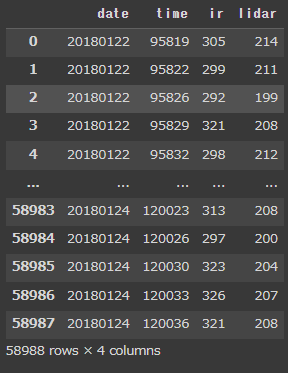
\includegraphics[width=.3\linewidth]{img/1.png}
    \caption{実行結果}
    \label{j1}
    \end{center}
  \end{figure}
  例えば、\verb|"lidar"| 列の0 $\sim$ 5番目の要素を抜き出して表示する場合は、ソースコード\ref{s2}\cite{robo}を実行する。実行結果を図\ref{j2}に示す。
  \begin{lstlisting}[caption=要素の抜き出し表示,label=s2]
print(data["lidar"][0:5])
  \end{lstlisting}
  \begin{figure}[htbp]
    \begin{center}
    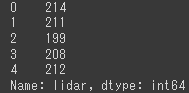
\includegraphics[width=.3\linewidth]{img/2.png}
    \caption{実行結果}
    \label{j2}
    \end{center}
  \end{figure}

  ヒストグラムの描画はソースコード\ref{s3}\cite{robo}を実行する。実行結果を図\ref{j3}に示す。
  \begin{lstlisting}[caption=ヒストグラムの描画,label=s3]
import matplotlib.pyplot as plt # 描画モジュールのインポート
data["lidar"].hist(bins = max(data["lidar"]) - min(data["lidar"]),align='left')
# ヒストグラムのピン数をセンサデータの最大値と最小値の差に設定
plt.show() # 描画    
  \end{lstlisting}

  \begin{figure}[htbp]
    \begin{center}
    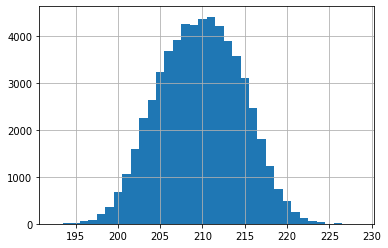
\includegraphics[width=.7\linewidth]{img/3.png}
    \caption{実行結果}
    \label{j3}
    \end{center}
  \end{figure}

このヒストグラムから、以下の3点を読み取ることができる。
\begin{itemize}
  \setlength{\parskip}{0cm} % 段落間
  \setlength{\itemsep}{0cm} % 項目間
  \item $194 \verb|~| 226 \mathrm{\,[mm]}$までの範囲の値が得られた。
  \item $210 \mathrm{\,[mm]}$付近の頻度が高い。
  \item 高頻度の部分からセンサ値が左右に離れるほど頻度が低くなる。
\end{itemize}


\mysubsection{ノイズの数値化}
前項より、センサデータの特徴が明らかになった。
ここでは、センサデータのノイズの傾向を数値化する。
具体的には、ノイズの平均値、分散、標準偏差を求める。
\verb|data["lidar"]|の平均値を、式\eqref{zlidar}に表す。
\begin{equation}
  z_{\rm{LiDAR}} = \{z_i|i = 0, 1, 2, ..., N-1\} \label{zlidar}  
\end{equation}
ここで、$z_{\rm{LiDAR}}$の平均値$\mu$は、式\eqref{meanz}で与えられる。
\begin{equation}
  \mu = \frac{1}{N}\sum_{i=0}^{N-1} z_i \label{meanz}
\end{equation}\\
これをソースコード\ref{s4}のように実装する。
なお、\verb|mean1| の計算は、平均値の定義に基づいており、
\verb|mean2|の計算は、\verb|pandas| の平均を求める \verb|mean| メソッドを利用している。
ソースコード\ref{s4}\cite{robo}に実装を示す。
実行結果を図\ref{j4}に示す。
\begin{lstlisting}[caption=平均値の計算,label=s4]
mean1 = sum(data["lidar"].values)/len(data["lidar"].values)
mean2 = data["lidar"].mean()
print(mean1,mean2)
\end{lstlisting}

\begin{figure}[htbp]
  \begin{center}
  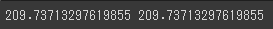
\includegraphics[width=.5\linewidth]{img/4.png}
  \caption{実行結果}
  \label{j4}
  \end{center}
\end{figure}

ソースコード\ref{s5}\cite{robo}のように実装することで、
ヒストグラム上に平均値を出力する。
実行結果を図\ref{s5}に示す。
\begin{lstlisting}[caption=平均値の出力,label=s5]
data["lidar"].hist(bins = max(data["lidar"]) - min(data["lidar"]),color="orange",align='left')   ###avgplot###
plt.vlines(mean1,ymin=0,ymax=5000,color="red")
plt.show()
\end{lstlisting}

\begin{figure}[htbp]
  \begin{center}
  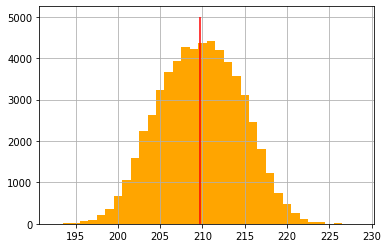
\includegraphics[width=.7\linewidth]{img/5.png}
  \caption{実行結果}
  \label{j5}
  \end{center}
\end{figure}

\mysubsubsection{分散}
次に分散を求める。標本分散は、式\eqref{h_bunsan}で定義される。
\begin{equation}
  \label{h_bunsan}
  \sigma^2 = \frac{1}{N}\sum_{i=0}^{N-1} (z_i - \mu)^2 (N > 0)
\end{equation}\\
各値と平均値の差の二乗値は、各値と平均値が離れているほど大きくなるため、分散は、リストの値が互いに大きく異なる程大きくなる。この問題を解決するために、不偏分散が式\eqref{f_bunsan}で定義される。
\begin{equation}
  \label{f_bunsan}
  \sigma^2 = \frac{1}{N-1}\sum_{i=0}^{N-1}(z_i - \mu)^2 (N>1)
\end{equation}\\
これらの分散をソースコード\ref{s6}\cite{robo}のように実装する。
分散の計算モジュールとして、python には、\verb|pandas|と\verb|numpy|が挙げられる。
それぞれ、実装の考え方が異なり、\verb|pandas| は不偏分散を、\verb|numpy| は標本分散を元に実装されている。実行結果を図\ref{j6}に示す。

\begin{lstlisting}[caption=分散の計算,label=s6]
# 定義から計算                      ### calcvar
zs = data["lidar"].values  
mean = sum(zs)/len(zs)
diff_square = [ (z - mean)**2 for z in zs]

sampling_var = sum(diff_square)/(len(zs))     # 標本分散
unbiased_var = sum(diff_square)/(len(zs)-1) # 不偏分散

print(sampling_var)
print(unbiased_var)

# Pandasを使用
pandas_sampling_var = data["lidar"].var(ddof=False) # 標本分散
pandas_default_var = data["lidar"].var()        # デフォルト(不偏分散)

print(pandas_sampling_var)
print(pandas_default_var)

# NumPyを使用
import numpy as np

numpy_default_var = np.var(data["lidar"])  # デフォルト(標本分散)
numpy_unbiased_var = np.var(data["lidar"], ddof=1)  # 不偏分散

print(numpy_default_var)
print(numpy_unbiased_var)
\end{lstlisting}


\begin{figure}[htbp]
  \begin{center}
  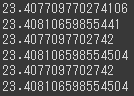
\includegraphics[width=.3\linewidth]{img/6.png}
  \caption{実行結果}
  \label{j6}
  \end{center}
\end{figure}

\mysubsubsection{標準偏差}
標準偏差を求める。標準偏差は、分散の平方根であるため、
ソースコード\ref{s7}\cite{robo}のようにして実装できる。\verb|pandas|では、\verb|std|メソッドを使ってデータから標準偏差を求めることができる。
実行結果を図\ref{j7}に示す。
\begin{lstlisting}[caption=標準偏差の計算,label=s7]
import math ###  calcstddev

# 定義から計算
stddev1 = math.sqrt(sampling_var)
stddev2 = math.sqrt(unbiased_var)
 
# Pandas を使用 
pandas_stddev = data["lidar"].std()
  
print(stddev1)
print(stddev2)
print(pandas_stddev)
\end{lstlisting}

\begin{figure}[htbp]
  \begin{center}
  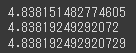
\includegraphics[width=.3\linewidth]{img/7.png}
  \caption{実行結果}
  \label{j7}
  \end{center}
\end{figure}

センサデータの誤差の傾向は、標準偏差を用いて説明することができる。
今回の場合、平均値が$209.7\mathrm{\,[mm]}$で、 標準偏差が$\pm 4.8 \mathrm{\,[mm]}$で誤差が生じることになる。


\mysubsubsection{確率分布}
続いて、センサデータのリスト$z_{\rm{LiDAR}} = \{z_i|i = 0, 1, 2,..., N-1\}$から、$N$回目以降に取得されるセンサ値$z_N, z_{N+1}...$を予想する問題を考える。直観的には、ヒストグラムの頻度の大きい値が出やすいと予測できる。これを数値化したものを仮に確率として定義する。
つまり、0回目から$N-1$回目まで記録されたセンサデータにあるデータ$z$が$m$個含まれていたら、その値の出る確率を$P(z) = m/N$と考えることを指す。
まず、各センサデータの頻度を集計する。ソースコード\ref{s8}\cite{robo}に実装を示す。実行結果を図\ref{j8}に示す。

\begin{lstlisting}[caption=センサデータの頻度の集計,label=s8]
freqs = pd.DataFrame(data["lidar"].value_counts())  # DataFrame関数のvalue_counts()メソッドを用いて、出現頻度の大きい順に配列データに格納する。
freqs.transpose() # 横向きに出力
\end{lstlisting}

\begin{figure}[htbp]
  \begin{center}
  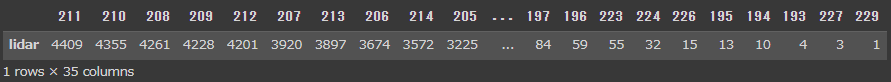
\includegraphics[width=\linewidth]{img/8.png}
  \caption{実行結果}
  \label{j8}
  \end{center}
\end{figure}

その後、確率の列を追加する。ソースコード\ref{s9}\cite{robo}に実装を示す。
\begin{lstlisting}[caption=確率の列の追加,label=s9]
freqs["probs"] = freqs["lidar"]/len(data["lidar"]) # 確率: "lidar" 列に入っているそれぞれの頻度を dataの要素数で割る。
freqs.transpose()  
\end{lstlisting}

\begin{figure}[htbp]
  \begin{center}
  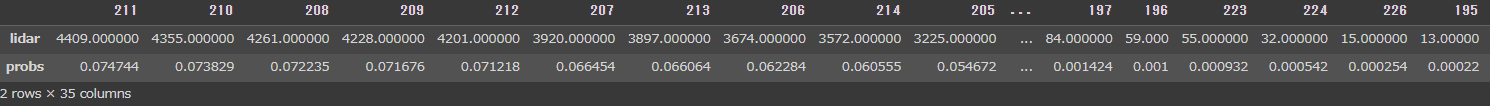
\includegraphics[width=\linewidth]{img/9.png}
  \caption{実行結果}
  \label{j9}
  \end{center}
\end{figure}

出力から、最頻出のセンサデータは、211で、0.075程度の確率で発生と分かる。
さらに、出力結果をセンサデータで並び変えて、横軸にセンサ軸、縦軸に確率を描くことで
確率質量関数を得る。各変数に対して、確率がどのように分布するかを表す$P$を確率分布と呼ぶ。
確率質量関数の実装をソースコード\ref{s10}\cite{robo}に示す。実行結果を図\ref{j10}に示す。

\begin{lstlisting}[caption=センサデータの並び替え,label=s10]
freqs["probs"].sort_index().plot.bar()   # 確率を距離の小さい順に並び替え
plt.show()
\end{lstlisting}

\begin{figure}[htbp]
  \begin{center}
  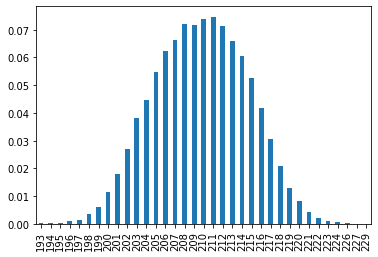
\includegraphics[width=.7\linewidth]{img/10.png}
  \caption{実行結果}
  \label{j10}
  \end{center}
\end{figure}

確率分布が求まったため、ソフトウェアでセンサデータの発生をシミュレーションすることができる。
以下のように実装する。
\verb|sample| メソッドを使うことで、確率分布から値を選ぶことができる。
ソースコード\ref{s11}\cite{robo}に実装を示す。実行結果を図\ref{j11}に示す。
\begin{lstlisting}[caption=センサデータのシミュレーション,label=s11]
def drawing(): #関数として定義  ###one_sampling###
  return freqs.sample(n=1, weights="probs").index[0]
drawing() # 実行
\end{lstlisting}

\begin{figure}[htbp]
  \begin{center}
  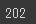
\includegraphics[width=.1\linewidth]{img/11.png}
  \caption{実行結果}
  \label{j11}
  \end{center}
\end{figure}

\mysubsubsection{正規分布}
以前の結果より、センサデータのばらつきが正規分布に従うことが分かる。
センサデータは、整数の値のみの離散的な値しかとらないが、連続的な値を取得できるものと仮定する。
センサデータ$z$が、$a$以上$b$未満に入る確率を式\eqref{pz}で定義する。
正規分布を式\eqref{gauss_bunpu}に示す。

\begin{align}
  P(a \leq z < b) = \int_{a}^{b} p(z) dz \label{pz} \\
  p(z) = \frac{1}{\sqrt{2\pi\sigma^2}}\exp \left\{-\frac{(z-\mu)^2}{2\sigma^2}\right\} \label{gauss_bunpu}
\end{align}
\\
$\sigma^2$ は分散、$\mu$は平均値である。
先ほど求めたセンサデータの平均値 $\mu = 209.7 \mathrm{\,[mm]}$、分散 $\sigma^2 = 23.4$ を代入して式\eqref{gauss_bunpu}を描画する。
ソースコード\ref{s12}\cite{robo}に実装を示す。実行結果を図\ref{j12}に示す。

\begin{lstlisting}[caption=センサデータの正規分布の描画,label=s12]
def p(z, mu=209.7, dev=23.4):   ###pdf_from_def###
  return math.exp(-(z - mu)**2/(2*dev))/math.sqrt(2*math.pi*dev) #math 関数による正規分布の実装
zs = range(190,230)   ###pdf_plot_from_def###
ys = [p(z) for z in zs]

plt.plot(zs,ys)
plt.show()
\end{lstlisting}

\begin{figure}[htbp]
  \begin{center}
  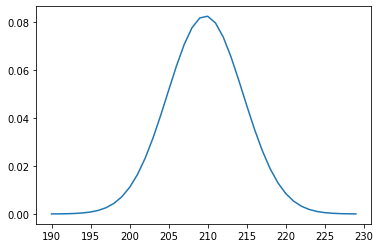
\includegraphics[width=.7\linewidth]{img/12.png}
  \caption{実行結果}
  \label{j12}
  \end{center}
\end{figure}